\chapter{Global Validation: The Massless Hadronic \texorpdfstring{$R$}{R}-Ratio}\label{ch:validation}

The antenna functions constructed and integrated in Chapter~\ref{ch:workedexample} are now
subjected to a global validation through the calculation of the massless hadronic $R$-ratio up to
NNLO. This fully inclusive observable provides a particularly stringent test of the antenna set,
since the different real and virtual contributions enter at each perturbative order and their
infrared poles must cancel in the inclusive sum, as discussed in
Chapter~\ref{ch:physicsbackground}. The resulting finite NLO and NNLO coefficients can then be
compared with the known $R$-ratio results obtained independently using methods other than antenna
subtraction \cite{Dine:1979qh}.

\section{The Hadronic $R$-Ratio}\label{sec:rratioDef}

The hadronic $R$-ratio is defined as the ratio of the total cross section for electron--positron
annihilation into hadrons to the point-like cross section for muon-pair production,
\begin{equation}
    \begin{split}
        R_\text{had} &= \frac{\sigma(e^+e^-\to\text{hadrons})}{\sigma(e^+e^-\to\mu^+\mu^-)}\\
          &= \frac{3q^2}{4\pi\alpha_\text{em}^2}\,\sigma(e^+e^-\to\text{hadrons}).
    \end{split}
\end{equation}
For massless quarks, the hadronic cross section can be related, through the optical theorem, to the
imaginary part of the electromagnetic current correlator
\cite{GehrmannDeRidder0311276,Adler1974}. Equivalently, its perturbative evaluation can be organised
as an inclusive sum over the partonic final states produced by the virtual photon. This makes the
$R$-ratio particularly well suited to the global validation performed in this chapter. At leading
order, the hadronic $R$-ratio is \cite{Ellis:1996mzs},
\begin{equation}
    R^{(0)} = N\sum_q e_q^2,
\end{equation}
where the sum runs over the active quark flavours and $e_q$ denotes the quark electric charge in
units of the positron charge. It is convenient to factor out this Born-level contribution and define
\begin{equation}
    R_\text{had} = R^{(0)}R(\alpha_s),
\end{equation}
where the normalised ratio admits the perturbative expansion,
\begin{equation}
    R(\alpha_s) = 1 + \frac{\alpha_s}{2\pi}\,r_\text{NLO} + \left(\frac{\alpha_s}{2\pi}\right)^2 r_\text{NNLO} + \mathcal O\!\left(\alpha_s^3\right).
\end{equation}
At each perturbative order, the coefficients $r_\text{NLO}$ and $r_\text{NNLO}$ receive contributions
from partonic final states of different multiplicities and loop orders. In the antenna formulation
used in this work, these contributions are expressed in terms of the corresponding integrated antenna
functions derived in Chapter~\ref{ch:workedexample}. At NLO, the real and virtual contributions
involve $\mathcal A_3^0$ and $\mathcal A_2^1$, respectively, while at NNLO the complete set of two-,
three-, and four-parton contributions is required.

The normalised quantity $R(\alpha_s)$ will be reconstructed from these integrated antenna functions
in the following sections and compared with the known result obtained independently using methods
other than antenna subtraction \cite{Dine:1979qh}.

\section{Assembly from Integrated Antenna Functions}\label{subsec:Tobjects}

The antenna functions constructed in Chapter~\ref{ch:workedexample} are colour-stripped kinematic
quantities. To reconstruct the contributions to the inclusive hadronic rate, the antennae associated
with each partonic final state must therefore be combined with the appropriate colour factors and
normalisation. In this work, these colour-restored, final-state-specific combinations are denoted by
$T$-objects.

The notation for a $T$-object identifies both the corresponding partonic final state and its
perturbative order. The subscript specifies the final-state particles, while the superscript denotes
the perturbative order, with $2$, $4$, and $6$ corresponding to LO, NLO, and NNLO, respectively. The
LO two-parton contribution, associated with the process $\gamma^*\to q\bar q$, provides the common
normalisation and is given by
\begin{equation}
    T_{q\bar q}^2 = N\left|\mathcal M_2^0\right|^2 = 4N(1-\epsilon)q^2.
\end{equation}
For convenience, we define
\begin{equation}
    P = 2C_FT_{q\bar q}^2.
\end{equation}
At NLO, the inclusive rate receives contributions from the virtual two-parton process
$\gamma^*\to q\bar q$ and the real-emission three-parton process $\gamma^*\to q\bar q g$. In terms of
the corresponding antenna functions, their $T$-objects are
\begin{equation}
    T_{q\bar q}^4 = P\,A_2^1,\qquad
    T_{q\bar qg}^4 = P\,A_3^0.
\end{equation}
At NNLO, contributions arise from two-, three-, and four-parton final states. The two-parton
contribution contains the different colour components of the two-loop antenna set, together with the
one-loop-squared contribution,
\begin{equation}
    T_{q\bar q}^6 = P\left(NA_2^2+\frac1N\tilde A_2^2+N_f\hat A_2^2+\left(N-\frac1N\right)\breve A_2^2\right).
\end{equation}
The three-parton real--virtual contribution is
\begin{equation}
    T_{q\bar qg}^6 = P\left[N\!\left(A_3^1+A_2^1A_3^0\right)-\frac1N\!\left(\tilde A_3^1+A_2^1A_3^0\right)+N_f\hat A_3^1\right].
\end{equation}
Finally, the four-parton double-real contributions are separated according to their partonic final
states,
\begin{equation}
    T_{q\bar qq^\prime\bar q^\prime}^6 = P\,(N_f-1)B_4^0,
\end{equation}
\begin{equation}
    T_{q\bar qq\bar q}^6 = P\left(B_4^0-\frac1N C_4^0\right),
\end{equation}
\begin{equation}
    T_{q\bar qgg}^6 = P\left(NA_4^0-\frac1N\tilde A_4^0\right).
\end{equation}
Upon integration over the corresponding final-state phase spaces, the antenna functions appearing in
these expressions are replaced by their integrated counterparts, $\mathcal A$, $\mathcal B$, and
$\mathcal C$, obtained in Chapter~\ref{ch:workedexample}. The only exceptions are $\tilde A_4^0$ and
$C_4^0$: their integrated counterparts are defined in the literature with an explicit overall factor
of $2$ and $\tfrac12$, respectively, and the corresponding terms of Eq.~\eqref{eq:rNNLO} therefore
carry the compensating factors $\tfrac12$ and $2$, as discussed in Section~\ref{sec:rratioNNLO}. We
denote the resulting integrated combinations by $\mathcal T$-objects. These quantities provide the individual two-, three-, and
four-parton contributions entering the inclusive $R$-ratio.

\iffalse

\subsection{Assembly from Integrated Antennae}\label{subsec:Tobjects}

Using \textit{AntCalc}, we are also able to compute the R-ratio step-by-step, without
having to resort to the automated function by just computing the intermediate steps
ourselves. As described in Subsection~\ref{subsec:colourAlg}, antenna functions are purely
kinematic. By taking all components, we are able to construct a process-wide
object carrying both kinematic and colour information. These are $T$-objects; their unintegrated
and integrated forms are denoted $T$ and $\mathcal T$, respectively. Conceptually,
the unintegrated $T$-object is defined as
\footnote{The $T$-objects are commonly notated by $T^2$, $T^4$ and $T^6$, depending
on their perturbative order: LO, NLO and NNLO, respectively. That is the same as
the $k$-index, introduced in Subsection~\ref{subsec:antennaFuncs} of Chapter~\ref{ch:physicsbackground}, incremented by one
and then doubled, $2(k+1)$. This
is the notation used in \cite{Gehrmann-DeRidder:2004ttg} and the one that will be
used for the rest of the present work.}
,
\begin{equation}
    T_\text{topology}^{2(k+1)}=\text{(colour/flavour weight)}\times T_{q\bar q}^2\times\text{(colour-weighted sum of antennae at $k$-order)}.
\end{equation}
This construction takes a simple form for the $A$-type antenna relative
$T$-objects \cite{Gehrmann-DeRidder:2005btv}:
\begin{equation}\label{eq:ATypeTObj}
    T_\text{topology}^{2(k+1)}=2C_F T_{q\bar q}^2\sum_{a} f_aA_{n, (k), a}^l
\end{equation}
where $a$ denotes the component (leading, subleading, fermion loop, etc), $f_a$
is the colour weight, that is $N$, $1/N$, $N_f$, etc, and $A_{n, (k), a}^l$ is the
relative component antenna with $n$ final-state particles and $l$ loops. For this
antenna type, this definition needs two extensions at NNLO that do not cleanly
fit into an algorithmic formula:
\begin{itemize}
    \item The $A_3^1$ antenna set represents a particularly interesting process.
    Unlike in lower order loop processes, here two very distinct kinds of
    Feynman diagram appear: those in which the loop and the emission of the
    final-state gluon are completely separate events, and those in which the
    loop involves all three external legs. The first kind of diagram maps exactly
    a $A_2^1$ antenna topology followed by a $A_3^0$ topology: first the two hard
    quarks exchange a gluon and then one of the hard quarks emits a final-state
    gluon\footnote{This is merely a conceptual, diagrammatic interpretation,
    as the actual process is much less sequential than this description suggests.}.
    Since this behaviour is not unique to the $A_3^1$ antenna, it must
    be subtracted from the bare result to retain the antenna's singular behaviour.
    When we then reconstruct the $T$-object, the $A_2^1A_3^0$ term has to be
    added back on such that the process is considered in its totality \cite{Gehrmann-DeRidder:2005btv}.
    \item The $A_2^2$ antenna set, also at NNLO, is the first time we find a
    double-loop topology. Here the extension required is not a subtraction of
    some kind of behaviour, but rather an addition of a new one. This set is, in
    reality, composed of two different processes: the first follows the standard
    rule closely, as it produces a leading, a subleading and a fermion loop
    component. The second, however, has a singular antenna which describes the
    self-interference of the one-loop correction with itself, now that the system
    presents with two loops.
    This antenna is denoted by $\breve A_2^2$. It is also the only
    genuinely square (not cross) term at NNLO. This means that it requires a
    normalisation of $(2C_F)^2$ \cite{Gehrmann-DeRidder:2005btv}.
\end{itemize}

As mentioned before, Eq.~\eqref{eq:ATypeTObj} is only valid for
$T$-objects constructed from $A$-type antenna functions. In this work we consider
all quark-antiquark antennae up to NNLO. This includes the $B_4^0$ and $C_4^0$ antennae
introduced in Subsection~\ref{subsec:antFamilies} of Chapter~\ref{ch:physicsbackground}. These
antennae populate the $T_{q\bar qq^\prime\bar q^\prime}^6$ and $T_{q\bar qq\bar q}^6$
objects, respectively.

$T_{q\bar qq^\prime\bar q^\prime}^6$ is built in the same way as other single-topology
antenna $T$-objects, like $T_{q\bar qg}^4$, with the only difference being that
here all quark flavours are summed over, requiring the inclusion of a $(N_f-1)$
term, constructing,
\begin{equation}
    T_{q\bar qq^\prime\bar q^\prime}^6=2C_FT_{q\bar q}^2(N_f-1)B_4^0.
\end{equation}
The identical-flavour quark-antiquark-quark-antiquark final state is described by
the sum of antennae for non-identical-flavour and for identical-flavour-only
\cite{Gehrmann-DeRidder:2005btv}. Using Eq.~\eqref{eq:genTSum} in the interference
term, with the identity piece vanishing by tracelessness,
we can describe the
identical-flavour $T$-object as,
\begin{equation}
    T_{q\bar q q\bar q}^6 = 2C_FT_{q\bar q}^2\left[B_4^0-\frac1N C_4^0\right]
\end{equation}
importantly without the inclusion of the quark-flavour sum term $(N_f-1)$.

With this definition of the integrated antenna $\mathcal X_n^l$ (Eq.~\eqref{eq:antennaIntegral}
of Chapter~\ref{ch:physicsbackground}), we are now also able to introduce the often used
integrated $T$-object as,
\begin{equation}\label{eq:integratedT}
    \mathcal T_\text{topology}^{2(k+1)} = 2C_FT_{q\bar q}^2\sum_a f_a \mathcal X_{n,(k),a}^l
\end{equation}
written schematically from Eq.~\eqref{eq:ATypeTObj}, though the structure may change
with the antenna type used to define the relevant $T$-object. This equation describes
that the integrated $T$-object, $\mathcal T_\text{topology}^{2(k+1)}$ is defined
using the integrated antennae $\mathcal X_n^l$, integrated over their respective
phase-spaces rather than integrating the composite unintegrated $T$-object directly
\cite{Gehrmann-DeRidder:2005btv,Gehrmann-DeRidder:2004ttg}.

\fi

\section{NLO Validation}\label{sec:rratioNLO}

At NLO, the inclusive hadronic $R$-ratio receives contributions from the virtual correction to the
two-parton final state, $\gamma^*\to q\bar q$, and from the real-emission process,
$\gamma^*\to q\bar q g$. In terms of the integrated antenna functions obtained in
Chapter~\ref{ch:workedexample}, these contributions are described by $\mathcal A_2^1$ and
$\mathcal A_3^0$, respectively. Using the $T$-object normalisation introduced in the previous
section, the NLO coefficient can therefore be written as
\begin{equation}
    \begin{gathered}
        r_\text{NLO} = \frac{\mathcal T_{q\bar q}^4+\mathcal T_{q\bar qg}^4}{T_{q\bar q}^2} = 2C_F\left(\mathcal A_2^1 + \mathcal A_3^0\right)\\
        = 2C_F\left[\left(-\frac{1}{\epsilon^2}-\frac{3}{2\epsilon}-4+\frac{7\pi^2}{12}+\ldots\right)+\left(\frac{1}{\epsilon^2}+\frac3{2\epsilon}+\frac{19}4-\frac{7\pi^2}{12}+\ldots\right)\right]=\frac32 C_F.
    \end{gathered}
\end{equation}
Thus, the $1/\epsilon^2$ and $1/\epsilon$ infrared poles of the virtual contribution cancel exactly
against those generated by the integrated real-emission contribution, as required for the inclusive
observable. This cancellation provides a first global check of the relative normalisation and
combination of the integrated antenna functions. For $N=3$, where $C_F=4/3$, the NLO contribution
becomes,
\begin{equation}
    \frac{\alpha_s}{2\pi}\,\frac{3}{2}C_F=\frac{\alpha_s}{\pi},
\end{equation}
reproducing the standard NLO correction to the massless hadronic $R$-ratio.

\section{NNLO Validation and the Hadronic $R$-Ratio}\label{sec:rratioNNLO}

At NNLO, the global validation requires the simultaneous combination of the double-virtual
two-parton, real--virtual three-parton, and double-real four-parton contributions. In contrast to the
NLO case discussed above, several colour structures and partonic final states contribute. Using the
integrated $\mathcal T$-objects defined in Section~\ref{subsec:Tobjects}, the normalised hadronic
$R$-ratio can be assembled order by order as,
\begin{equation}
    \begin{split}
        R(\alpha_s) ={}& 1 + \frac{\alpha_s}{2\pi}\frac{\mathcal T_{q\bar q}^4+\mathcal T_{q\bar qg}^4}{T_{q\bar q}^2}\\
                       &+ \left(\frac{\alpha_s}{2\pi}\right)^2\frac{\mathcal T_{q\bar q}^6+\mathcal T_{q\bar qg}^6+\mathcal T_{q\bar q q\bar q}^6+\mathcal T_{q\bar q q^\prime\bar q^\prime}^6+\mathcal T_{q\bar q gg}^6}{T_{q\bar q}^2} + \mathcal O\!\left(\alpha_s^3\right)\\
                       ={}& 1 + \frac{\alpha_s}{2\pi}r_\text{NLO} + \left(\frac{\alpha_s}{2\pi}\right)^2r_\text{NNLO} + \mathcal O\!\left(\alpha_s^3\right).
    \end{split}
\end{equation}
The NNLO coefficient therefore tests the complete massless antenna set calculated in
Chapter~\ref{ch:workedexample}. Substituting the definitions of the $T$-objects, it can be expressed
entirely in terms of the corresponding integrated antenna functions,
\begin{equation}\label{eq:rNNLO}
    \begin{split}
        r_\text{NNLO} = 2C_F\,\Bigg[&N\!\left(\mathcal A_2^1\mathcal A_3^0+\mathcal A_3^1+\mathcal A_4^0+\mathcal A_2^2\right)-\frac1N\!\Big(\mathcal A_2^1\mathcal A_3^0+\tilde{\mathcal A}_3^1+\tfrac12\tilde{\mathcal A}_4^0+2\,\mathcal C_4^0-\tilde{\mathcal A}_2^2\Big)\\
                                    &+N_f\!\left(\mathcal B_4^0+\hat{\mathcal A}_3^1+\hat{\mathcal A}_2^2\right)+2C_F\breve{\mathcal A}_2^2\Bigg].
    \end{split}
\end{equation}
The factors $\tfrac12$ and $2$ multiplying $\tilde{\mathcal A}_4^0$ and $\mathcal C_4^0$ follow from the
definitions of these integrated antennae in the literature. In $\tilde A_4^0$ the two gluons are
photon-like, coupling only to the quark and antiquark, so that, unlike the colour-ordered $A_4^0$, which
is a sum of two ordered sub-antennae, it is a sum of four sub-antennae that give identical integrals over
the tripole phase space (Eqs.~(5.27) and (5.28) of Ref.~\cite{Gehrmann-DeRidder:2005btv}). Its integrated
expression therefore carries an explicit overall factor of $2$ (Eq.~(5.32) of
Ref.~\cite{Gehrmann-DeRidder:2005btv}), whereas the inclusive $q\bar qgg$ contribution to the $R$-ratio
contains exactly half of it (Eq.~(4.53) of Ref.~\cite{Gehrmann-DeRidder:2004ttg}), which gives
$\tfrac12\tilde{\mathcal A}_4^0$. Likewise, $C_4^0$ is the identical-flavour-only interference term and
its integrated expression carries an explicit factor of $\tfrac12$ (Eq.~(5.44) of
Ref.~\cite{Gehrmann-DeRidder:2005btv}), whereas the identical-flavour four-quark contribution to the
$R$-ratio contains twice this value (Eq.~(4.51) of Ref.~\cite{Gehrmann-DeRidder:2004ttg}), which gives
$2\,\mathcal C_4^0$. The integrated antennae computed with \textit{AntCalc} in
Chapter~\ref{ch:workedexample} follow these literature definitions, including the explicit factors.

Each contribution in Eq.~\eqref{eq:rNNLO} is individually infrared divergent. After inserting the
integrated antenna functions obtained in Chapter~\ref{ch:workedexample}, however, the poles cancel in
the sum. In particular, the coefficients of
\begin{equation*}
    \frac1{\epsilon^4},\qquad\frac1{\epsilon^3},\qquad\frac1{\epsilon^2},\qquad\frac1\epsilon
\end{equation*}
vanish, leaving a finite NNLO coefficient. This cancellation simultaneously tests the relative
normalisation, colour decomposition, and assembly of the two-, three-, and four-parton antenna
contributions.

Combining the finite NLO result of Section~\ref{sec:rratioNLO} with the NNLO contribution gives
\begin{equation}\label{eq:RfinalResult}
    R(\alpha_s) = 1+\frac{\alpha_s}{2\pi}\frac32C_F+\left(\frac{\alpha_s}{2\pi}\right)^2C_F\!\left[N\left(\frac{243}{16}-11\zeta_3\right)+\frac3{16N}+N_f\left(-\frac{11}4+2\zeta_3\right)\right]+\mathcal O\!\left(\alpha_s^3\right).
\end{equation}
The result is finite and agrees with the known massless hadronic $R$-ratio through NNLO
\cite{Gehrmann-DeRidder:2004ttg,Dine:1979qh}. Importantly, this comparison is with results obtained
independently of the antenna-subtraction construction used here. The agreement therefore provides a
global validation of the complete massless antenna set calculated in
Chapter~\ref{ch:workedexample}: not only do the infrared poles cancel when the different final-state
contributions are combined, but the remaining finite coefficient reproduces the independently known
inclusive result.

\section{Implementation in \textit{AntCalc}}\label{sec:rratioImpl}

The assembly of the hadronic $R$-ratio described in the previous sections is automated in
\textit{AntCalc} through the function \texttt{BuildRRatio}. For the massless QCD antenna set
considered in this work, the calculation is performed with \texttt{BuildRRatio[SMQCD]}.

The function performs the assembly described explicitly in Sections~\ref{subsec:Tobjects}--\ref{sec:rratioNNLO},
combining the integrated antenna contributions with their corresponding colour factors and
normalisations at each perturbative order. The cancellation of the infrared poles occurs within this
assembly, so that the returned result is finite through NNLO. The output of
\texttt{BuildRRatio[SMQCD]} therefore reproduces the analytic result obtained in
Eq.~\eqref{eq:RfinalResult}, which in turn agrees with the independently known massless hadronic
$R$-ratio through NNLO \cite{Gehrmann-DeRidder:2004ttg,Dine:1979qh}. This provides an automated global
check of both the integrated massless antenna set and its implementation in \textit{AntCalc}.

\section{Comparison with Experimental Data}\label{sec:rratioData}

As an additional illustration of the perturbative result obtained above, the \textit{AntCalc}
prediction for the hadronic $R$-ratio can be compared with the experimental data compiled by the
Particle Data Group (PDG) \cite{Tanabashi:2018oca}. Figure~\ref{fig:rratioFullDomain} shows this
comparison over a broad range of centre-of-mass energies. The purpose of this comparison is not to
describe the full experimental spectrum. The result derived in this work is a massless fixed-order
perturbative QCD prediction and therefore does not include several effects that are important in
specific energy regions. At low energies, the data exhibit pronounced hadronic resonance and
non-perturbative structure. Heavy-quark thresholds and quarkonium resonances also produce features
that are not described by the massless approximation, while at energies around the $Z$ pole
electroweak contributions dominate the observed behaviour. Consequently, agreement with the data
should only be expected away from such regions, where a fixed-order perturbative description is
appropriate.

\begin{figure}[h!]
    \centering
    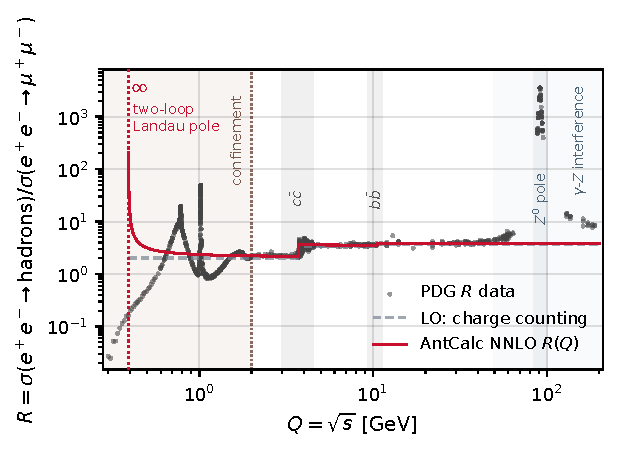
\includegraphics[width=0.8\textwidth]{figures/rratio-full-domain.pdf}
    \caption{Comparison of the massless NNLO $R$-ratio obtained with \textit{AntCalc} with the PDG data over the full energy range considered. The LO charge-counting result is shown for reference. The indicated regions highlight the low-energy non-perturbative regime, heavy-quark thresholds, and the electroweak $Z^0$-pole region, illustrating the limited domain in which the massless fixed-order QCD prediction can be meaningfully compared with the data.}
    \label{fig:rratioFullDomain}
\end{figure}

Figure~\ref{fig:rratioContinuumOrders} focuses on the energy range
$2\lesssim\sqrt{s}\lesssim30\,\mathrm{GeV}$, where the comparison with the massless perturbative QCD
prediction is more informative. The charm- and bottom-quark threshold regions, where the massless
approximation is not expected to provide an adequate description, are indicated by the grey-shaded
bands. Away from these regions, the inclusion of higher-order QCD corrections improves the overall
description of the experimental data relative to the LO prediction. This is particularly visible in
the lower panel, where the results are normalised to the LO prediction and the NLO and NNLO curves
are generally shifted towards the experimental measurements. Moreover, the relatively small change
from NLO to NNLO compared with that from LO to NLO is indicative of good convergence of the
perturbative expansion in this energy range.

\begin{figure}[h!]
    \centering
    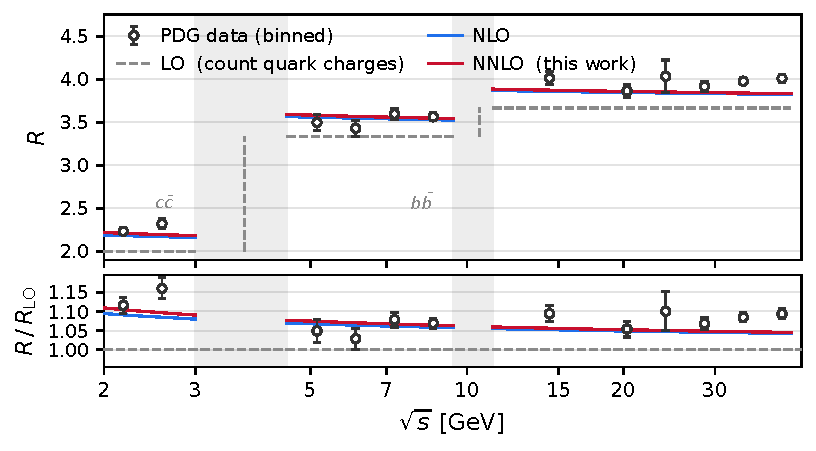
\includegraphics[width=0.8\textwidth]{figures/rratio_talk.pdf}
    \caption{Comparison of the LO, NLO, and NNLO massless perturbative predictions for the hadronic $R$-ratio with the PDG data in the range $2\lesssim\sqrt{s}\lesssim30\,\mathrm{GeV}$. The grey-shaded bands indicate the charm- and bottom-quark threshold regions. The lower panel shows the results normalised to the LO prediction, highlighting the improved overall description obtained after including the higher-order QCD corrections.}
    \label{fig:rratioContinuumOrders}
\end{figure}

\section{Summary}

The massless antenna functions calculated in Chapter~\ref{ch:workedexample} have been subjected to a
global validation through the hadronic $R$-ratio. At both NLO and NNLO, the infrared poles of the
individual real and virtual contributions cancel in the inclusive sum, providing a stringent check of
the relative normalisation, colour structure, and assembly of the integrated antenna functions. The
resulting finite coefficients reproduce the known massless hadronic $R$-ratio through NNLO,
previously obtained using methods independent of antenna subtraction
\cite{Gehrmann-DeRidder:2004ttg,Dine:1979qh}. This agreement therefore confirms not only the internal
consistency of the antenna set, but also its consistency with independently established QCD results.

The comparison with the PDG data provides an additional phenomenological illustration of the
calculation. In the energy region where the massless fixed-order approximation is applicable, and away
from the heavy-quark threshold regions, the inclusion of successive perturbative orders generally
improves the agreement between the theoretical prediction and the experimental measurements. Moreover,
the comparatively small shift from NLO to NNLO relative to that from LO to NLO is indicative of good
convergence of the perturbative expansion in this region. Conversely, the deviations observed in
regions dominated by non-perturbative, heavy-quark threshold, resonance, or electroweak effects
illustrate the expected limitations of the massless fixed-order approximation.

Taken together, the cancellation of the infrared poles, the agreement with the independently known
perturbative $R$-ratio, and the comparison with experimental data provide complementary checks of the
results obtained in this work. In particular, the first two constitute the principal global validation
of the complete massless antenna set implemented in \textit{AntCalc} through NNLO. This validation is
especially important because these antenna functions are intended to serve as building blocks for the
construction of subtraction terms in NNLO QCD calculations: their successful combination in a physical
inclusive observable provides a non-trivial test of their relative normalisation, colour structure,
and integrated infrared behaviour. The comparison with experimental data further illustrates the
phenomenological behaviour of the resulting prediction within the expected domain of applicability of
the massless fixed-order approximation.
